
\subsection{Principe de décomposition}

\subsection{Principe de modélisation autonome}

Un autre principe que nous souhaitons développer est celui de la
séparation maximale des étapes du processus.

Comme nous l'expliquions dans le \autoref{chap:2} deux étapes sont
nécessaires pour transformer une position décrite en une \emph{zone de
  localisation probable,} la \emph{spatialisation} et la
\emph{fusion.} Mais ces deux étapes peuvent être combinées
différemment.

Une première solution consiste à \enquote{chainer} la
\emph{spatialisation} des différents \emph{indices de localisation,}
comme on peut le voir sur la figure \ref{fig:comp_approches_lin}. Avec
cette approche les différentes \emph{zones de localisation
  compatibles} sont créées les unes à la suite des autres, ainsi la
zone de recherche en entrée de chaque étape de \emph{spatialisation}
dépend des \emph{spatialisations} précédentes. Avec cette approche,
l'opération de \emph{fusion} est implicite, elle s'opère, en partie, à
chaque nouvelle \emph{spatialisation,} puisque les zones ne
correspondant pas aux \emph{indices de localisation} sont retirées peu
à peu. La \emph{zone de localisation probable,} en bleu sur la figure
\ref{fig:comp_approches}, est obtenue une fois que l'on a
\emph{spatialisé} tous les \emph{indices de localisation.} Cette
approche est la première que nous ayons envisagée. Elle a pour
avantage d'être simple à concevoir et à développer. Cependant cette
approche à un problème majeur. À cause de l'enchainement des étapes de
\emph{spatialisation} les erreurs se répercutent d'une étape à
l'autre. Ainsi, si un des \emph{indices de localisation} est mal
\emph{spatialisé}, que ce soit à cause de la méthode utilisée ou d'une
mauvaise description, cela se répercute sur toutes les
\emph{spatialisations} ultérieures. La moindre correction impose donc
de refaire l'ensemble des traitements.

Une seconde solution, plus robuste, consiste à effectuer l'ensemble
des opérations de \emph{spatialisation} en parallèle, comme le montre
la figure \ref{fig:comp_approches_sep}. Avec cette approche la
\emph{spatialisation} des différents \emph{indices de localisation}
est effectuée séparément et leur \emph{fusion} est effectuée dans un
second temps. Comme pour la démarche \enquote{chainée} une
\emph{spatialisation} erronée peut impacter la \emph{zone de
  localisation probable,} toutefois il est plus facile de corriger ces
erreurs. En effet, si les différentes \emph{zones de localisation
  compatibles} ont été conservées il est possible de faire une
nouvelle \emph{fusion} en retirant un, ou plusieurs \emph{indices de
  localisation.} Alors qu'avec une approche \enquote{chainée} il est
nécessaire de refaire toutes les opérations de \emph{spatialisations}
ultérieures à celle de \emph{l'indice de localisation} que l'on
souhaite modifier ou retirer et ce même si les résultats
intermédiaires ont été conservés.

\begin{figure}
  \centering
  \subfloat[Construction suivant une démarche linéaire]{
    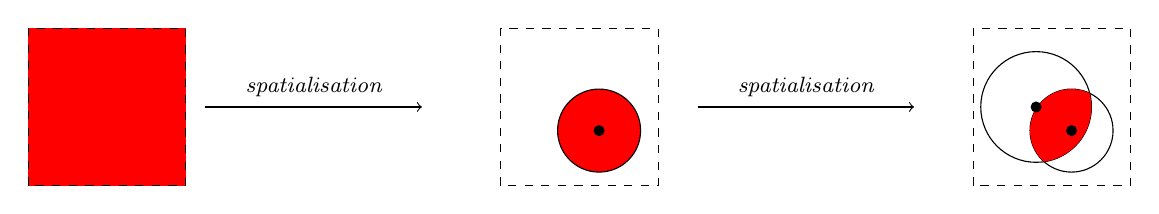
\begin{tikzpicture}

  \begin{scope}
    \path[fill=red] (0,0) rectangle (2,2);
	\path[draw, dashed] (0,0) rectangle (2,2);
  \end{scope}

  \path[draw, ->] (2.25,1) --++ (2.75,0)  node[pos=.5, above] {\footnotesize \itshape spatialisation};

  \begin{scope}[xshift=6cm]
	\path[draw, dashed] (0,0) rectangle (2,2);
	\begin{scope}
	    \begin{scope}
	      \clip (0,0) rectangle (2,2);
	      \fill[red] (1.25,.7) circle [radius=15pt];
	      \path[draw] (1.25,.7) circle [radius=15pt];
	    \end{scope}
	\end{scope}
    \node[circle, inner sep=0pt,minimum size=4pt, fill] (c) at (1.25,.7)
    {};
  \end{scope}



  \path[draw, ->] (8.5,1) --++ (2.75,0)  node[pos=.5, above] {\footnotesize \itshape spatialisation};




  \begin{scope}[xshift=12cm]
	\path[draw, dashed] (0,0) rectangle (2,2);
	\path[draw] (1.25,.7) circle [radius=15pt];
    \path[draw](.8,1) circle [radius=20pt];
	\begin{scope}
	    \begin{scope}
	      \clip (1.25,.7) circle [radius=15pt];
	      \fill[red] (.8,1) circle [radius=20pt];
	    \end{scope}
	\end{scope}
    \node[circle, inner sep=0pt,minimum size=4pt, fill] (c) at (1.25,.7)
    {};
    \node[circle, inner sep=0pt,minimum size=4pt, fill] (c) at (.8,1)
    {};
  \end{scope}


\end{tikzpicture}
    \label{fig:comp_approches_lin}
  }

  \subfloat[Construction suivant une démarche autonome]{
    \begin{tikzpicture}

  \begin{scope}
    \path[ffa] (0,0) rectangle (2,2);
    \path[ffc] (0,0) rectangle (2,2);
  \end{scope}

  \path[draw, ->] (2.25,1) --++ (2.75,1.5)  node[pos=.5, above] {\footnotesize \itshape spatialisation};
  \path[draw, ->] (2.25,1) --++ (2.75,-1.5)  node[pos=.5, above] {\footnotesize \itshape spatialisation};

  \begin{scope}[xshift=6cm, yshift=-1.5cm]
    \path[draw, dashed] (0,0) rectangle (2,2);
    \begin{scope}
      \begin{scope}
        \clip (0,0) rectangle (2,2);
        \fill[ffa] (1.25,.7) circle [radius=15pt];
        \path[ffc] (1.25,.7) circle [radius=15pt];
      \end{scope}
    \end{scope}
    \node[circle, inner sep=0pt,minimum size=4pt, fill] (c) at (1.25,.7)
    {};
  \end{scope}

  \begin{scope}[xshift=6cm,yshift=1.5cm]
    \path[draw, dashed] (0,0) rectangle (2,2);
    \fill[ffa](.8,1) circle [radius=20pt];
    \path[ffc](.8,1) circle [radius=20pt];
    \node[circle, inner sep=0pt,minimum size=4pt, fill] (c) at (.8,1)
    {};
  \end{scope}

  \path[draw, ->] (8.5,1) --++ (2.75,0)  node[pos=.5, above] {\footnotesize \itshape fusion};


  \begin{scope}[xshift=12cm]
    \path[draw,dashed] (0,0) rectangle (2,2);
    \path[draw,dashed] (1.25,.7) circle [radius=15pt];
    \path[draw,dashed](.8,1) circle [radius=20pt];
    \begin{scope}
      \begin{scope}
        \clip (1.25,.7) circle [radius=15pt];
        \fill[ffa2] (.8,1) circle [radius=20pt];
        \path[ffc2] (.8,1) circle [radius=20pt];
      \end{scope}
      \begin{scope}
        \clip (.8,1) circle [radius=20pt];
        \path[ffc2] (1.25,.7) circle [radius=15pt];
      \end{scope}
    \end{scope}
    \node[circle, inner sep=0pt,minimum size=4pt, fill] (c) at (1.25,.7)
    {};
    \node[circle, inner sep=0pt,minimum size=4pt, fill] (c) at (.8,1)
    {};
  \end{scope}


\end{tikzpicture}
    \label{fig:comp_approches_sep}
  }
  \caption{Comparaison du processus de construction de la \emph{zone
      de localisation probable} pour une alerte à deux \emph{indices
      de localisation}.}
  \label{fig:comp_approches}
\end{figure}

Le principe de modélisation autonome peut, de plus, tirer parti du
principe de décomposition précédemment présenté.

% Justifier choix

\subsection{Principe de modélisation non bivalente}

\subsection{Principe de modélisation explicite des connaissances}

\subsection{Principe d'intégration dans le contexte métier}

\subsection{Principe de raisonnement en monde ouvert}


Comme le montre la figure \ref{fig:md_ferme} dans \emph{l'hypothèse du
  monde clos} toute règle inconnue est considérée comme fausse. Alors
que dans \emph{l'hypothèse du monde ouvert} (Figure
\ref{fig:md_ouvert}) les règles inconnues sont considérées comme
telles, \ie que l'on estime qu'elles peuvent être vraies, comme
fausses.

Pour illustrer la différence entre ces deux hypothèses on peut prendre
l'exemple suivant. Imaginons que je décrive le contenu de ma
bibliothèque de la suivante : \enquote{Dans ma bibliothèque on trouve
  les ouvrages : \emph{méthodes de logique,} de Willard \bsc{Quine} et
  \emph{le projet \emph{Cybersyn},} d'Eden \bsc{Medina}.} Cette phrase
peut être décomposée en deux assertions logiques, \enquote{ma
  bibliothèque contient l'ouvrage \emph{méthodes de logique}} et
\enquote{ma bibliothèque contient l'ouvrage \emph{le projet
    \emph{Cybersyn}}.} Avec \emph{l'hypothèse du monde clos} toute
autre proposition logique est considérée comme fause, ainsi à la
question \enquote{Est-ce que tu as tel livre ?} (à l'exception deux
précédemment mentionnés) la réponse sera toujours \enquote{non}, dans
ce contexte cela revient à considérer que j'ai donné une description
exhaustive du contenu de ma bibliothèque. Avec \emph{l'hypothèse du
  monde ouvert} on considère que les règles qui nous sont inconnues
peuvent être vraies ou fausses, ainsi, dans ce cadre on ne peut que
répondre \enquote{Je ne sais pas} à la question précédente. Dans
\emph{l'hypothèse d'un monde ouvert,} l’absence d'une règle n'implique
pas sa fausseté.

\begin{figure}
  \centering
  \subfloat[Illustration de l'hypothèse du monde clos]{
    \begin{tikzpicture}
  \begin{scope}
    \fill[ffa] (1,.75) arc(90:270:.75) -- cycle;% [radius=.75cm];
    \path[ffc] (1,.75) arc(90:270:.75) -- cycle;
    \node[color=RdBu-9-1] at (.625,0) {V};
  \end{scope}
  \begin{scope}
    \fill[ffa2] (1,1) arc(270:90:-1) -- cycle;% [radius=.75cm];
    \path[ffc2] (1,1) arc(270:90:-1) -- cycle;
    \node[color=RdBu-9-9] at (1.375,0) {F};
  \end{scope}
  \begin{scope}
    \path[ffc, draw=black] (1,0) circle [radius=.75cm];
  \end{scope}
  \begin{scope}
    \node (rect) [anchor=north, minimum width=.5cm,minimum
    height=.25cm,ffc, draw=black] at (0,-1.25) {};
    \node[anchor=west, font=\tiny\vphantom{Ag}, text width = 4cm] at
    ([xshift=1ex]rect.east) {Connues};
    
    \node (rect2) [anchor=north, minimum width=.5cm,minimum
    height=.25cm, ffa, ffc] at ([yshift=-.25cm]rect) {};
    \node[anchor=west, font=\tiny\vphantom{Ag}, text width = 4cm] at
    ([xshift=1ex]rect2.east) {Vraies};
    
    \node (rect3) [anchor=north, minimum width=.5cm,minimum
    height=.25cm, ffa2, ffc2] at ([yshift=-.25cm]rect2) {};
    \node[anchor=west, font=\tiny\vphantom{Ag}, text width = 4cm] at
    ([xshift=1ex]rect3.east) {Fausses};
    
    \draw[decorate,decoration={brace}] ([xshift=7.75ex]rect.north
    east) -- ([xshift=7.75ex]rect3.south east);
    \node[anchor=west, font=\tiny\vphantom{Ag}, text width = 2cm] at
    ([xshift=8ex]rect2.east) {Ensemble des règles};   
  \end{scope}
\end{tikzpicture}
    \label{fig:md_ferme}
  }\hspace{3cm}
  \subfloat[Illustration de l'hypothèse du monde ouvert]{
    \begin{tikzpicture}
  \begin{scope}
    \fill[ffa] (1,1) arc(90:270:1) -- cycle;% [radius=.75cm];
    \path[ffc] (1,1) arc(90:270:1) -- cycle;
    \node[color=RdBu-9-1] at (.625,0) {V};
  \end{scope}
  \begin{scope}
    \fill[ffa2] (1,1) arc(270:90:-1) -- cycle;% [radius=.75cm];
    \path[ffc2] (1,1) arc(270:90:-1) -- cycle;
    \node[color=RdBu-9-9] at (1.375,0) {F};
  \end{scope}
  \begin{scope}
    \path[ffc, draw=black] (1,0) circle [radius=.75cm];
    \node[text width=3cm] (leg) at (4,1)
    {\footnotesize \itshape Ensemble des règles connues};
    \path[draw, ->] (leg.west) --++ (25:-.9);
  \end{scope}
\end{tikzpicture}
    \label{fig:md_ouvert}
  }
  \caption{Illustration des hypothèses du \emph{monde clos} et du
    \emph{monde ouvert}}
  \label{fig:comp_md}
\end{figure}


%%% Local Variables:
%%% mode: latex
%%% TeX-master: "../../../../main"
%%% End:
